% 气体分子对容器壁的压强
% 分子|理想气体|碰撞|压强|容器壁

\pentry{动量定理\upref{PLaw}}

我们来从微观的角度考察气体是如何对一个光滑平面产生压强的. 一种错误的解释是: 每个气体分子像一个有弹性的小球, 他们互紧挨着, 对彼此和容器壁产生压力, 当体积越小, 压力也就越大. 然而真实情况\footnote{除了极端温度或压强的情况}是, 气体分子之间的距离远远大于他们的体积, 且都在不断运动. 是大量分子撞击容器壁产生的 “冲击力” 对容器产生了等效的压力. 这种撞击可以看作是在一瞬间完成的, 就像高中学的完全弹性碰撞. 所以我们需要使用动量和冲量, 而不是作用力.

\begin{figure}[ht]
\centering
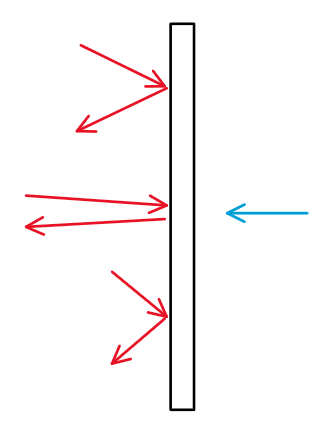
\includegraphics[width=3cm]{./figures/MolPre_1.png}
\caption{分子对容器壁的压强} \label{MolPre_fig1}
\end{figure}

如\autoref{MolPre_fig1}, 我们假设空间中没有重力, 向右为 $x$ 方向, 一块面积为 $S$ 的光滑平板初始时静止, 令其质量为 $M$, 远大于分子的质量. 平板的左侧不断受到大量粒子从各个随机方向,以各种随机速度的撞击. 虽然每个分子的动量很小, 但撞击的频率却很大(数量级与阿伏伽德罗常数相当, 即 $10^{24}$ 次每秒). 由于这些撞击的位置完全是随机的, 他们可以被等效为一个均匀的压强. 如何定义等效压强呢? 我们可以在平板的右侧对平板施加一个均匀恒定的 “真正的” 压强 $P$ (或者等效地, 直接施加恒力 $F = PS$), 如果左边分子的撞击和右边的压强能使平板保持宏观的静止, 那么我们就说分子撞击对平板的(等效)压强为 $P$.

我们给这些分子编号, 假设第 $i$ 个分子延 $x$ 方向的速度分量为 $v_{x,i}$, 质量都为 $m$, 则碰撞前延 $x$ 方向的动量为 $p_i = m v_{x,i}$. 由于平板的质量远大于单个分子的质量, 撞击以后可以认为分子 $x$ 方向的速度取相反数, 而平行于平板方向的速度不变(类似于光的镜面反射). 这样, 碰撞后单个分子的动量变化(即冲量)为 $\Delta p_i = -2mv_{x,i}$, 由动量守恒, 平板的动量瞬间增加了 $2mv_{x,i}$. 如果一段时间 $\Delta t$ 内, 有 $N$ 个分子撞击平板, 则平板受到向右的总冲量为
\begin{equation}
\Delta p = \sum_{i=1}^N 2mv_{x,i} = 2m \sum_{i=1}^N v_{x,i}
\end{equation}
再来看右边的压力对平板的作用. $\Delta t$ 时间内该作用力对平板向左的冲量为
\begin{equation}\label{MolPre_eq1}
\Delta p = PS \Delta t
\end{equation}
若要使平板在宏观上不动, 总冲量必须为零, 以上两式相等, 即
\begin{equation}
P = \frac{2m}{S\Delta t} \sum_{i=1}^N v_{x,i} = 2m\bar v_{x,i} \frac{N}{S\Delta t}
\end{equation}
其中我们定义 $x$ 方向速度平均值为
\begin{equation}\label{MolPre_eq2}
\bar v_{x,i} = \frac{1}{N}\sum_{i=1}^N v_{x,i}
\end{equation}
也就是说, 等效压强和分子在垂直容器壁方向的平均动量成正比, 与单位面积单位时间撞击容器壁的粒子数成正比.

\subsection{两块平板}
我们再来讨论一个稍微复杂一些的情况. 假设空间中有两块平行平板, 他们之间距离为 $a$, 每个粒子会在这两块平板之间来回反弹(假设不飞出边界), 第 $i$ 个粒子来回运动一次的周期是 $T_i = 2a/v_{x,i}$, $\Delta t$ 时间(假设远大于 $T_i$)内可以与右边的平板发生碰撞的次数为
\begin{equation}
N_i = \frac{\Delta t}{T_i} = \frac{v_{x,i} \Delta t}{2a}
\end{equation}
所有的分子在 $\Delta t$ 时间内碰撞右壁的次数为 $N = \sum N_i$.

所以 $\Delta t$ 时间内, 右侧平板获得的总冲量为
\begin{equation}\label{MolPre_eq3}
\Delta p = \sum_{i=1}^N 2mv_{x,i} N_i = \frac{m \Delta t}{a} \sum_{i=1}^N v_{x,i}^2 = m\overline {v_{x,i}^2} \frac{ N\Delta t}{a}
\end{equation}
其中我们定义了速度平方得平均值(注意这与\autoref{MolPre_eq2} 的平方 $\bar v_{x,i}^2$ 不同)
\begin{equation}
\overline {v_{x,i}^2} = \frac{1}{N} \sum_{i=1}^N v_{x,i}^2
\end{equation}
与上面同理, 为了保持总冲量相等, \autoref{MolPre_eq3} 和\autoref{MolPre_eq1} 必须相等, 得
\begin{equation}\label{MolPre_eq4}
P = m \overline {v_{x,i}^2} \frac{N}{Sa}
\end{equation}

从这个公式出发, 我们很容易可以得到理想气体状态方程\upref{PVnRT}. 注意这里的 $Sa$ 就是两平板之间的体积, 而 $mv_{x,i}^2$ 就是单个分子动能 $E_{k,i}$ 的两倍.
